\documentclass{article}
\usepackage{tikz}
\usepackage[acronym]{glossaries}
\usetikzlibrary{positioning}
\usetikzlibrary{arrows}
\usetikzlibrary{shapes.misc}
\usetikzlibrary{shapes}
\usepackage[
  language=auto,%
  style=numeric-comp,%
  sorting=nyt, % name, year, title
  maxbibnames=10, % default: 3, et al.
  backend=biber,
  natbib=true % natbib compatibility mode (\citep and \citet still work)
]{biblatex}

\newacronym{SuV}{SuV}{System under Verification}
\newacronym{SuO}{SuO}{System under Observation}
\newacronym{RV}{RV}{Runtime verification}
\newacronym{PSL}{PSL}{Property Specification Language}
\newacronym{SERE}{SERE}{Sequential Regular Expression}
\newacronym{LTL}{LTL}{Linear Temporal Logic}

\newacronym{DFA}{DFA}{Deterministic finite automata}
\newacronym{NFA}{NFA}{Non-deterministic finite automata}
\newacronym{TCB}{TCB}{Trusted Code Base}

\newacronym{HDL}{HDL}{Hardware Description Language}
\newacronym{FM}{FM}{Formal methods}
\newacronym{FV}{FV}{Formal verification}

\newacronym{BSV}{BSV}{Bluespec SystemVerilog}

\newacronym{DSL}{DSL}{Domain Specific Language}
\newacronym{eDSL}{eDSL}{Embedded Domain Specific Language}
\newacronym{LOC}{LOC}{Lines of Code}
\newacronym{STA}{STA}{Static Timing Analysis}

\newacronym{GADT}{GADT}{Generalized Algebraic Data Type}
\newacronym{ADT}{ADT}{Algebraic Data Type}

\newacronym{CPU}{CPU}{Central Processing Unit}
\newacronym{GPU}{GPU}{Graphics Processing Unit}
\newacronym{GPGPU}{GPGPU}{General Purpose Graphics Processing Unit}

% \newacronym{NIDS}{NIDS}{Network Intrusion Detection System}
\newacronym{PLA}{PLA}{Programmable Logic Array}
\newacronym{FOSS}{FOSS}{Free and Open Source Software}
\newacronym{REPL}{REPL}{Read-Eval-Print-Loop}
\newacronym{IP}{IP}{Intellectual Property}

%% \newacronym[
%%     \glslongpluralkey={Regular expressions},
%%     \glsshortpluralkey={regexes}
%%   ]{TaA}{regex}{regular expression}

\newacronym[
    \glslongpluralkey={Regular expressions},
    \glsshortpluralkey={regexes}
  ]{rgx}{regex}{regular expression}

%% % \newacronym[
%% %     \glslongpluralkey={Tests-as-atoms regexes},
%% %     \glsshortpluralkey={T-regexes}
%% %   ]{TaA}{T-regex}{Tests-as-atoms regex}

%% \newacronym[
%%     \glslongpluralkey={Regular expressions},
%%     \glsshortpluralkey={regexes}
%%   ]{regex}{regex}{Regular expression}

\newacronym{EDA}{EDA}{Electronic Design Automation}
\newacronym{FPGA}{FPGA}{Field Programmable Gate Array}
\newacronym{ASIC}{ASIC}{Application Specific Integrated Circuit}
\newacronym{SSD}{SSD}{Solid State Drive}
\newacronym{GHC}{GHC}{Glasgow Haskell Compiler}
\newacronym{VHDL}{VHDL}{VHSIC Hardware Description Language}
\newacronym{LUT}{LUT}{Look-up table}
% \newacronym{AC}{AC}{Air conditioning system}
\newacronym{RAM}{RAM}{Random Access Memory}

\newcommand{\bvec}{Boolean vector}
\newcommand{\bvecs}{Boolean vectors}

% \newglossaryentry{TaA}{
%   name=T-regex,
%   description={Tests-as-atoms regex},
%   plural=T-regexes
% }

% \newglossaryentry{regex}{
%   name=regex,
%   description={Regular expression},
%   plural=regexes
% }

% \newglossaryentry{EDA}{
%   name=EDA,
%   description={Electronic Design Automation}
% }

% \newglossaryentry{FPGA}{
%   name=FPGA,
%   description={Field Programmable Gate Array}
% }

% \newglossaryentry{ASIC}{
%   name=FPGA,
%   description={Application Specific Integrated Circuit}
% }

% \newglossaryentry{SSD}{
%   name=SSD,
%   description={Solid State Drive}
% }

% \newglossaryentry{GHC}{
%   name=GHC,
%   description={Glasgow Haskell Compiler}
% }

% \newglossaryentry{VHDL}{
%   name=VHDL,
%   description={VHSIC Hardware Description Language}
% }

% \newglossaryentry{LUT}{
%   name=LUT,
%   description={Look-up table}
% }

% \newglossaryentry{AC}{
%   name=AC,
%   description={Air conditioning system}
% }


%\date{\today}
%\author{Julin Shaji}
\date{}
\author{}
\title{Towards verified regular expression matchers in hardware}
\addbibresource{../bibliography.bib}

\begin{document}
\maketitle

\section{Motivation}
This work is about producing hardware implementations of regular
expression matchers from within the theorem prover Coq.
% interactive theorem prover, namely Coq.
%in formally verifiable way.
Regular expression matching is used in a wide variety of
applications ranging from compilers to computational biology.
Our interest in regular expression matching stems from \emph{runtime
verification}, which is used to ensure correctness of reactive
systems.
%  enhance confidence in correctness of
% reactive systems.
Runtime verification involves the design and use of a \emph{monitor}
which observes the behaviour of a running system and flags deviations
from a formal specification describing its intended behaviour.
% to ensure that a running
% system is behaving as expected.
% The correct system behaviour is encoded as a formal specification.
% An entity named monitor observes the running system's observable
% behaviour and flags deviations from its specification.
% in which an entity named monitor
% is used Formal verification where a
% This is a form of formal 
%
% Formal verification is an effective technique to enhance confidence in
% correctness of such systems.
% Runtime verification is a dynamic form of Formal verification where a
% monitor is employed to check whether the system is correct with
% respect to a correctness property.
% expressing intended
% behaviour.
% Correctness properties used in Runtime verification need to be written in a formal
% language.
%
% Runtime verification entrusts the monitor with ensuring system
% correctness.
Effectiveness of runtime verification depends on the correctness of
the monitor.
Hence, the confidence in overall system correctness can be enhanced if
the monitor is proven correct.
%
% Properties of this kind need to be written in a formal language based
% on a temporal logic.
% %
% Regex can be helpful in writing such properties.


Specifications used in runtime verification are usually written in a
formal language based on a temporal logic.
% In this work, we provide a workflow by which hardware implementations
% of matchers for a generalized form of regular expressions may be
% generated from the Coq proof assistant.
We are interested in regular expression matching because of its use in
one such language named \emph{\gls{PSL}}.
This language is commonly used to write correctness specifications in
hardware verification.
%
% \gls{PSL} is such a language popular in the domain of hardware
% verification.
% Our work is a step towards the generation of verifiable \gls{PSL}
% checkers.
%
Properties in \gls{PSL} can be written using a generalized form of
regular expressions.
% called \glspl{SERE}.
% The atoms are Boolean \emph{tests} on the input alphabet rather than
% elements of the alphabet themselves.
%
% Hence, a verifiably correct monitor for specifications written in
% \gls{PSL} needs a verifiable regular expression matcher.
Hence, a monitor for specifications written in \gls{PSL} needs a
regular expression matcher.
%
% The regular expressions that we consider are essentially a subset of
% \gls{SERE} and are much more expressive and powerful when compared to
% classic regular expressions.
% The regular expressions that we consider are much more expressive and
% powerful when compared to classic regular expressions.
%
% In this thesis, we build a workflow by which matchers for a subset of
% \gls{SERE} may be generated as hardware implementations.
% Though we do not yet offer a correctness proof of our conversion
% procedure, the matchers are generated within the Coq proof assistant
% which makes it possible to construct correctness proofs in future.
Our work provides a mechanism which accepts a generalized form of
regular expressions within Coq and produces the hardware
implementation of a corresponding matcher.

\section{Generation of hardware from Coq}
The overall flow by which we produce hardware matcher from the input
regular expression may be divided into three stages as shown in
Fig.~\ref{fig:flow}.

\begin{enumerate}
\item
  Expressing the regular expression and generating corresponding NFA
  within Coq.
\item
  Converting Coq to Haskell code and using the extracted Haskell
  to produce equivalent Verilog.
\item 
  Applying EDA on the Verilog description to create FPGA bitstream.
\end{enumerate}

% Coq, HDL, HW impl
%

We capture the AST of regular expressions as a type within Coq.
Values of this type correspond to regular expressions.
% Regular expressions are represented by values of a type in Coq.
%
Our implementation of the McNaughton-Yameda
algorithm~\cite{mcnaughton1960regular} converts the input regular
expression to a corresponding NFA within Coq.
%
% Such values are 
% with our implementation of the McNaughton-Yameda
% algorithm~\cite{mcnaughton1960regular} within Coq.
%
% Given a regular expression, we utilize a function that we have written
% in Coq to build a corresponding NFA using the McNaughton-Yameda
% algorithm~\cite{mcnaughton1960regular}.
The NFA thus generated corresponds to the desired matcher.
%
We provide an \emph{\gls{eDSL}} as syntactic sugar to express regular
expressions in Coq.
%
% Since the regular expression values within Coq are verbose and hence
% tedious to write manually, we provide an \emph{\gls{eDSL}} with a
% friendly syntax to write them.
This \gls{eDSL} is made using Coq's notation mechanism.
% and implicitly
% converts regular expressions written in it to values of the regular
% expression type in Coq.
%
% The input regular expression is given within Coq by means of an
% \gls{eDSL} made using Coq's notation system.
% We use an \gls{DSL} embedded within Coq to provide the input regular
% expression to our flow.
% This \gls{DSL} is made using the notation mechanism of Coq and
% implicitly converts the regular expression to a Coq term. 
% The input regular expression is entered within Coq via an \gls{eDSL}.
% This provides a convenient way for users to provide the regular
% expression without being bogged down by the syntactical details of Coq.
% A term written in this \gls{eDSL} is automatically converted to a Coq value.
% We use a procedure written in Coq to produce an NFA corresponding to a
% matcher.
% This NFA is built using Thompson construction~\cite{thompson1968nfa}
% and is made in such a way that the language that it accepts is same as
% the one associated with the input regular expression.
% The matcher corresponding to this particular regular expression is generated as an
% NFA.
% This NFA is a term in Coq.

The NFA built within Coq needs to be converted to an HDL description
before its hardware implementation can be made.
Our approach is to use Coq's extraction procedure to convert the NFA
into Haskell code which is then converted to Verilog using the Clash
compiler.
% Having derived NFA for desired matcher within Coq, we need t
% Our aim is to produce hardware implementation of the matcher.
% As \gls{EDA} tools expect the input designs to be written in an HDL,
% we need to find a way to convert the NFA made in Coq to an HDL
% description.
% % Tools facilitating generation of hardware implementations expect
% % designs to be written in an HDL.
% % Hence, we need the NFA made within Coq as a description in Verilog or
% % VHDL.
% Though Coq supports conversion to languages like Haskell and OCaml by
% means of its extraction mechanism, there is no support for conversion
% to an HDL.
% We get around this limitation by using the ecosystem of a high-level
Clash~\cite{clash2010} is a high-level HDL 
based on the Haskell language.
Since valid Haskell code is also valid in Clash, we use the extracted
Haskell code to build a Clash design.
% This makes valid Haskell code also valid in Clash.
% The extracted 
% This allows us to use Coq's extraction feature to produce Haskell
% version of the NFA, which can then be used to build a Clash design.
We use a prewritten Haskell module to simulate the execution of the
extracted NFA by means of Thompson's algorithm~\cite{thompson1968nfa}.
The Clash compiler then converts the whole design to equivalent Verilog.
% Thus via extraction and the Clash compiler, we derive the Verilog
% description of the desired matcher.
Clash can generate synthesizable Verilog code only for a restricted
subset of Haskell.
%
% Note that the Clash compiler can convert only a subset of Haskell to
% synthesizable Verilog.
%
% is not capable of converting arbitrary
% Clash designs to Verilog , not all designs expressed in Clash are Clash places certain constraints on designs meant for
% synthesis.
We engineer our NFA construction in such a way that the Haskell code
extracted from Coq falls within this subset.
% Haskell satisfies these constraints.

The Verilog code generated with the help of Clash is converted to
corresponding FPGA bitstream using \gls{EDA} tools.
% We perform \gls{EDA} on the Verilog code generated from Clash to
% synthesize, place and route the design with respect to target FPGA.
% Finally, the appropriate bitstream is generated and loaded onto the
% FPGA.
The tools that we use for \gls{EDA} are open source, which leaves more
room for further modification and tweaking.
% using open source tools to produce an FPGA bitstream.
% Clash is an HDL using Haskell syntax. 
% Its compiler is capable of converting designs written in Haskell to
% equivalent Verilog.
% This gives us a pathway by which our NFA within Coq can be
% made into a Verilog design.
% First, the extraction mechanism of Coq is used to convert the Coq term
% corresponding to NFA to Haskell code that is compatible with
% Clash.
% We engineer the matcher construction so that the resultant design is
% synthesizable.
% The extracted Haskell is used to build a hardware design in Clash,
% which is then converted to Verilog using Clash compiler.
% Finally, synthesis and associated processes are performed using open
% source tools to produce FPGA bitstream.

\begin{figure}
  \centering
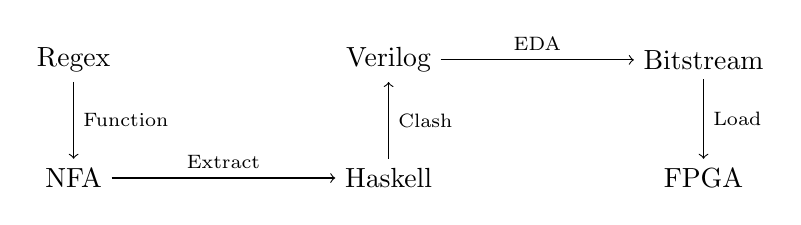
\begin{tikzpicture}
  \node (re) {Regex};
  \node[below of=re, yshift=-5mm] (nfa) {NFA};
  \node[right of=nfa, xshift=3cm] (hask) {Haskell};
  \node[above of=hask, yshift=5mm] (verilog) {Verilog};
  \node[right of=verilog, xshift=3cm] (bits) {Bitstream};
  \node[below of=bits, yshift=-5mm] (fpga) {FPGA};

  \draw[->] (re) -- (nfa) node[right,midway] {\scriptsize Function};
  \draw[->] (nfa) -- (hask) node[above,midway] {\scriptsize Extract};
  \draw[->] (hask) -- (verilog) node[right,midway] {\scriptsize Clash};
  \draw[->] (verilog) -- (bits) node[above,midway] {\scriptsize EDA};
  \draw[->] (bits) -- (fpga) node[right,midway] {\scriptsize Load};
\end{tikzpicture}
\caption{Overall flow}
\label{fig:flow}
\end{figure}

\section{Experimental results}
We used a GOWIN FPGA~\cite{gowinweb} to perform experimental
validation of our flow. 
%
The correctness of the generated Clash designs are checked using the
HedgeHog library~\cite{hedgehog} of Haskell, which performs
property-based testing.
% We took advantage of property-based testing to automatically check
% correctness of the generated Clash designs.
In addition, we perform simulation of the Verilog designs by means of
Verilator testbenches.
% We We also used verilator testbenches for simulation.

An important consideration in FPGA designs is resources used in terms
of LUTs and registers.
We observed that the resource utilization of the generated designs
increased linearly with respect to input regular expression size.
This is as expected since the number of states in an NFA grows
linearly with respect to the size of corresponding regular expression.
Thus, designs we generate are reasonably efficient.
% Thompson's algorithm.

We also study the time required for the overall flow.
The total time taken to produce matcher bitstream from input regular
expression appears to grow exponentially with respect to the size of
the regular expression.
% The NFA transition information is a sparse boolean matrix which leads
% to the HDL design size to grow rapidly, which in turn makes the tools
% take more time to process the designs.
% Despite this, the synthesis tool optimizes the design so that the
% utilization is low even for large regular expression size.
This is mostly due to the Haskell-Verilog conversion phase.
%
We were able to synthesize matchers for regular expressions with size
as large as 61 within 4 hours on an average desktop computer.
%
% Among the different phases of our flow, Haskell to Verilog generation
% takes up the most time.
% The nesting depth of the regular expression operations does not seem
% to have any effect on the FPGA resource utilization or time taken.
Note that the time taken to execute the flow is a one time cost and
hence is not as critical resource utilization.

\section{Conclusion}
% Despite the exponential increase in the total time taken for the flow
% to run,
% Though it takes a few hours for the entire flow to run for such large
% regular expressions,
The matchers that we build are for a generalized form of regular
expressions whose atoms are boolean functions.
Regular expressions useful for practical needs are small due to the
expressivity and power available due to this generalization.
%
For example, character classes can be represented with a single atom
using the regular expressions that we consider whereas it would take
as many characters as there are in the class for normal regular
expressions.
The matchers that our workflow generates are useful in monitoring
liveness properties for runtime verification.
%
% be satisfied by much
% smaller regular expressions as the kind of regular expressions we
% consider are very expressive.
%
% Also worth noting is that the time taken to produce the matcher is a
% one-time cost. Once the matcher is synthesized it can readily be used
% as often as needed.

% The regular expressions that we use are a generalized form of standard
% regular expressions.
% Boolean tests on input as
% atoms.
% Hence, they are more expressive and powerful than classic regular
% expressions.
% generate These regular expression are already useful to monitor liveness properties.
%Eg: burglary detection system

We build the matchers from within the Coq theorem prover.
Thus, we leave open the possibility of formally proving the
correctness of this construction.
We hope to build this proof as a follow-up to this work.


\printbibliography[heading=none]

\end{document}
